\documentclass[10pt,a4paper,twocolumn]{ltjsarticle}
\usepackage{luatexja-fontspec}
% 余白の設定
\usepackage[top=20truemm, bottom=24truemm, left=20truemm, right=20truemm]{geometry}

\usepackage{titlesec}
\titleformat*{\section}{\large}
\titleformat*{\subsection}{\large}

\usepackage{here}
\usepackage[luatex]{graphicx}
\usepackage{amsmath}
% \usepackage[ipa,deluxe]{luatexja-preset}

\usepackage{url}
\makeatletter
\newcommand*{\themonth}{\two@digits\month}
\newcommand*{\theday}{\two@digits\day}
\renewcommand{\today}{\the\year/\themonth/\theday}
\makeatother
\usepackage{fancyhdr}
\fancypagestyle{mypagestyle}{
  \lhead{\LaTeX サンプル (\today)}
  \rhead{Your Name}
  \renewcommand{\headrulewidth}{0.0pt}
}
\pagestyle{mypagestyle}

\begin{document}
\tableofcontents

\section{これはセクションです}
図\ref{lena_rgb}はlenaさんの画像です。
\begin{figure}[H]
  \centering
  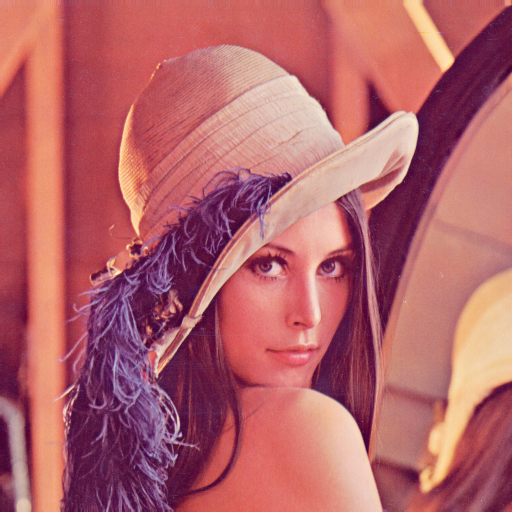
\includegraphics[width=6cm]{./lena.png}
  \caption{よくみる画像}
  \label{lena_rgb}
\end{figure}

\section{これは2つめのセクションです}
\subsection{これはサブセクションです}
\begin{figure}[H]
  \centering
  
\includegraphics[width=6cm]{./lena_gray.png}
  \caption{よくみる画像のグレースケール}
  \label{lena_gray}
\end{figure}

% http://www.latex-cmd.com/fig_tab/table01.html
\begin{table}[H]
  \centering
  \caption{牛丼メニュー}
  \label{table}
  \begin{tabular}{|l|c|r||r|} \hline
    メニュー & サイズ & 値段 & カロリー \\ \hline \hline
    牛丼 & 並盛 & 500円 & 600 kcal \\
    牛丼 & 大盛 & 1,000円 & 800 kcal \\
    牛丼 & 特盛 & 1,500円 & 1,000 kcal \\ \hline
    牛皿 & 並盛 & 300円 & 250 kcal \\
    牛皿 & 大盛 & 700円 & 300 kcal \\
    牛皿 & 特盛 & 1,000円 & 350 kcal \\ \hline
  \end{tabular}
\end{table}


数式が簡単にかけます。
\begin{eqnarray}
  && \iint_D f(x,y) dxdy \\
  && \iiint_D f(x,y) dxdy \\
  && \iiiint_D f(x,y) dxdy
\end{eqnarray}

引用\cite{Karras2018ASG}もできます。\cite{SALMAN2018221}
\bibliographystyle{unsrt}
\bibliography{references}

\end{document}
